\documentclass{article}
\usepackage{fullpage}
\usepackage[utf8]{inputenc}
\usepackage{pict2e}
\usepackage{amsmath}
\usepackage{enumitem}
\usepackage{eurosym}
\usepackage{mathtools}
\usepackage{amssymb, amsfonts, latexsym, cancel}
\setlength{\parskip}{0.3cm}
\usepackage{graphicx}
\usepackage{fontenc}
\usepackage{slashbox}
\usepackage{setspace}
\usepackage{gensymb}
\usepackage{accents}
\usepackage{adjustbox}
\setstretch{1.35}
\usepackage{bold-extra}
\usepackage[document]{ragged2e}
\usepackage{subcaption}
\usepackage{tcolorbox}
\usepackage{xcolor, colortbl}
\usepackage{wrapfig}
\usepackage{empheq}
\usepackage{array}
\usepackage{parskip}
\usepackage{arydshln}
\graphicspath{ {images/} }
\renewcommand*\contentsname{\color{black}Índice} 
\usepackage{array, multirow, multicol}
\definecolor{lightblue}{HTML}{007AFF}
\usepackage{color}
\usepackage{etoolbox}
\usepackage{listings}
\usepackage{mdframed}
\setlength{\parindent}{0pt}
\usepackage{underscore}
\usepackage{hyperref}
\usepackage{tikz}
\usepackage{tikz-cd}
\usetikzlibrary{shapes, positioning, patterns}
\usepackage{tikz-qtree}
\usepackage{biblatex}
\usepackage{pdfpages}
\usepackage{pgfplots}
\usepackage{pgfkeys}
\addbibresource{biblatex-examples.bib}
\usepackage[a4paper, left=1cm, right=1cm, top=1cm,
bottom=1.5cm]{geometry}
\usepackage{titlesec}
\usepackage{titletoc}
\usepackage{tikz-3dplot}
\usepackage{kbordermatrix}
\usetikzlibrary{decorations.pathreplacing}
\newcommand{\Ej}{\textcolor{lightblue}{\underline{Ejemplo}}}
\setlength{\fboxrule}{1.5pt}

% Configura el formato de las secciones utilizando titlesec
\titleformat{\section}
{\color{red}\normalfont\LARGE\bfseries}
{Tema \thesection:}
{10 pt}
{}

% Ajusta el formato de las entradas de la tabla de contenidos
\addtocontents{toc}{\protect\setcounter{tocdepth}{4}}
\addtocontents{toc}{\color{black}}

\titleformat{\subsection}
{\normalfont\Large\bfseries\color{red}}{\thesubsection)}{1em}{\color{lightblue}}

\titleformat{\subsubsection}
{\normalfont\large\bfseries\color{red}}{\thesubsubsection)}{1em}{\color{lightblue}}

\newcommand{\bboxed}[1]{\fcolorbox{lightblue}{lightblue!10}{$#1$}}
\newcommand{\rboxed}[1]{\fcolorbox{red}{red!10}{$#1$}}

\DeclareMathOperator{\N}{\mathbb{N}}
\DeclareMathOperator{\Z}{\mathbb{Z}}
\DeclareMathOperator{\R}{\mathbb{R}}
\DeclareMathOperator{\Q}{\mathbb{Q}}
\DeclareMathOperator{\K}{\mathbb{K}}
\DeclareMathOperator{\im}{\imath}
\DeclareMathOperator{\jm}{\jmath}
\DeclareMathOperator{\col}{\mathrm{Col}}
\DeclareMathOperator{\fil}{\mathrm{Fil}}
\DeclareMathOperator{\rg}{\mathrm{rg}}
\DeclareMathOperator{\nuc}{\mathrm{nuc}}
\DeclareMathOperator{\dimf}{\mathrm{dimFil}}
\DeclareMathOperator{\dimc}{\mathrm{dimCol}}
\DeclareMathOperator{\dimn}{\mathrm{dimnuc}}
\DeclareMathOperator{\dimr}{\mathrm{dimrg}}
\DeclareMathOperator{\dom}{\mathrm{Dom}}
\DeclareMathOperator{\infi}{\int_{-\infty}^{+\infty}}
\newcommand{\dint}[2]{\int_{#1}^{#2}}

\newcommand{\bu}[1]{\textcolor{lightblue}{\underline{#1}}}
\newcommand{\lb}[1]{\textcolor{lightblue}{#1}}
\newcommand{\db}[1]{\textcolor{blue}{#1}}
\newcommand{\rc}[1]{\textcolor{red}{#1}}
\newcommand{\tr}{^\intercal}

\renewcommand{\CancelColor}{\color{lightblue}}

\newcommand{\dx}{\:\mathrm{d}x}
\newcommand{\dt}{\:\mathrm{d}t}
\newcommand{\dy}{\:\mathrm{d}y}
\newcommand{\dz}{\:\mathrm{d}z}
\newcommand{\dth}{\:\mathrm{d}\theta}
\newcommand{\dr}{\:\mathrm{d}\rho}
\newcommand{\du}{\:\mathrm{d}u}
\newcommand{\dv}{\:\mathrm{d}v}
\newcommand{\tozero}[1]{\cancelto{0}{#1}}
\newcommand{\lbb}[2]{\textcolor{lightblue}{\underbracket[1pt]{\textcolor{black}{#1}}_{#2}}}
\newcommand{\dbb}[2]{\textcolor{blue}{\underbracket[1pt]{\textcolor{black}{#1}}_{#2}}}
\newcommand{\rub}[2]{\textcolor{red}{\underbracket[1pt]{\textcolor{black}{#1}}_{#2}}}

\author{Francisco Javier Mercader Martínez}
\date{}
\title{Visualización de Datos\\Informe Entregable Ejercicio 2}
\author{
\begin{tabular}{ll}
Francisco Javier Mercader Martínez & Rubén Gil Martínez\\
Javier Martínez Manresa & Francisco Barba Bernal\\ 
Guillermo López Pérez & 
\end{tabular}}
\usepackage{hyperref}
\hypersetup{
    colorlinks=true,
    linkcolor=black,
    urlcolor=blue,
}

\begin{document}
\maketitle
\textbf{\Large Actividad 1: Selección de la Visualización} 

El artículo seleccionado para utilizar como fuente de la visualización es el siguiente:
\begin{itemize}[label=\textbullet]
    \item Artículo: \textit{Principles of Effective Data Visualization}.
    \item Autor: Stephen R. Midway.
    \item Publicado en: \textit{Patterns}, Volumen 1, Diciembre 2020.
    \item DOI: \url{https://doi.org/10.1016/j.patter.2020.100141},
\end{itemize}
El artículo de Stephen R. Midway incluye varias visualizaciones que puede ser analizadas. Para este ejercicio, seleccionaremos la \textbf{Figura 1} del artículo, que presenta ejemplos de diferentes tipos de visualizaciones, como gráficos de barras, histogramas, diagramas de dispersión, mapas de calor, y gráficos de densidad. 

\textbf{\Large Actividad 2: Análisis Crítico del Diseño} 
\begin{center}
    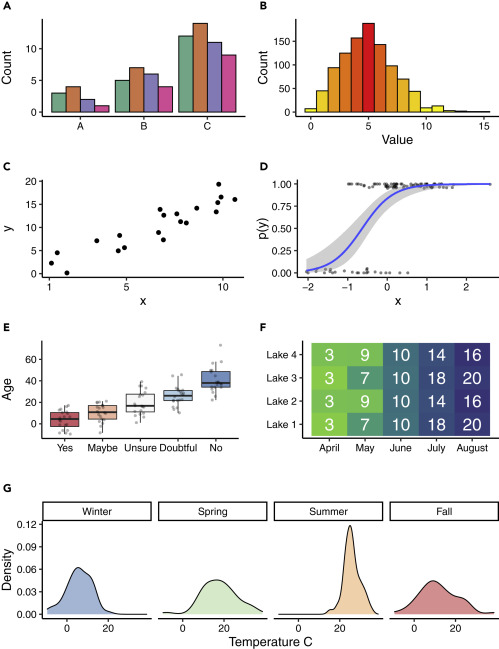
\includegraphics[width=0.4\textwidth]{Fig_1}\\
Figura 1: Visualización seleccionada
\end{center}

\textbf{Nivel 1: Dominio y Contexto}
\begin{itemize}[label=\textbullet]
    \item \textbf{Dominio:} La visualización pertenece al dominio de la comunicación científica y la visualización de datos.
    \item \textbf{Propósito principal:} Mostrar ejemplos de diferentes geometrías visuales y cómo estas pueden ser utilizadas para representar datos de manera efectiva.
    \item \textbf{Audiencia:} Científicos, investigadores y estudiantes interesados en mejorar sus habilidades de visualización de datos.
    \item \textbf{Necesidades informativas:} La audiencia necesita comprender cómo seleccionar y diseñar visualizacions que sean efectivas, claras y que transmitan el mensaje.
\end{itemize}
\textbf{Nivel 2: Abstracción de Tareas y Datos}
\begin{itemize}[label=\textbullet]
    \item \textbf{Tareas permitidas por la visualización:} 
        \begin{itemize}[label=\textbullet]
            \item Comparar distribuciones, con histogramas y gráficos de densidad, por ejemplo.
            \item Identificar relaciones entre variables, con el diagrama de dispersión.
            \item Analizar composiciones, con el mapa de calor.
        \end{itemize}
    \item \textbf{Tipos de datos presentados:}
        \begin{itemize}[label=\textbullet]
            \item Datos cuantitativos.
            \item Datos categóricos.
        \end{itemize}
    \item \textbf{Adecuación de la abstracción de tareas:} La visualización aborda adecuadamente las tareas al proporcionar ejemplos claros de cómo representar diferentes tipos de datos.
    \item \textbf{Representación visual:} La abstracción de datos permite una representación visual efectiva, ya que cada tipo de visualización está diseñada para un propósito específico, como los mencionados anteriormente. 
\end{itemize}
\textbf{Nivel 2: Idiomas de Codificación Visual e Interacción}
\begin{itemize}[label=\textbullet]
    \item \textbf{Marcas y canales utilizados:}
        \begin{itemize}[label=\textbullet]
            \item Marcas: Puntos, líneas, barras, áreas.
            \item Canales: Posición, longitud, color, saturación.
        \end{itemize}
    \item \textbf{Expresivididad:} La visualización expresa información relevante y evita elementos innecesarios.
    \item \textbf{Canales visuales:} Los canales están bien utilizados para los datos mostrados. Por ejemplo, el color se utiliza para representar la intensidad en el mapa de calor.
    \item \textbf{Principios de percepción visual:} Se respetan los colores diferenciados (discriminalidad), los graficos separados (agrupamiento) y el uso de diferentes colores para destacar (popout).
    \item \textbf{Idiomas de interacción:} La visualización es estática, por lo que no hay interacción. 
\end{itemize}
\textbf{Nivel 4: Algoritmos y Computación}
\begin{itemize}[label=\textbullet]
    \item \textbf{Algoritmos necesarios:} Para generar las visualizaciones, se podrían utilizar algoritmos de agrupamiento (para gráficos de barras agrupadas) y cálculo de densidad (para gráficos de densidad).
    \item \textbf{Problemas de rendimiento o escalabilidad:} No se identifican problemas importantes, ya que la figura muestra gráficos sencillos que no parecen haber necesitado cálculos complejos. 
\end{itemize}
\textbf{\Large Actividad 3: Amenazas a la Validez y Validación}

\textbf{Amenazas a la validez:}
\begin{itemize}[label=\textbullet]
    \item \textbf{Nivel 1 (Dominio y Contexto):}
        \begin{itemize}[label=\textbullet]
            \item Posible amenaza: Las personas que intenten interpretar los resultados que muestran las gráficas pueden no estar familiarizadas con algunos términos técnicos utilizados en las visualizaciones.
            \item Método de validación: Realizar entrevistas a los lectores del artículo para evaluar si han podido entenderlo.
        \end{itemize}
    \item \textbf{Nivel 2 (Abstracción de Tareas y Datos):}
        \begin{itemize}[label=\textbullet]
            \item Posible amenaza: Algunas visualizaciones, como el gráfico de barras, pueden no ser ideales para representar datos con incertidumbre (mencionado por el propio autor).
            \item Método de validación: Comparar la efectividad de diferentes geometrías para las mismas tareas.
        \end{itemize}
    \item \textbf{Nivel 3 (Idiomas de Codificación Visual e Interacción):}
        \begin{itemize}[label=\textbullet]
            \item Posible amenaza: Los colores utilizados en algunas visualizaciones pueden no se accesibles para personas con daltonismo.
        \end{itemize}
    \item \textbf{Nivel 4 (Algoritmos y Computación):} 
        \begin{itemize}[label=\textbullet]
            \item Posible amenaza: Si los datos fueran más complejos, podrían surgir problemas de escalabilidad.
            \item Método de validación: Realizar un análisis de la complejidad algorítmica.
        \end{itemize}
\end{itemize}
\textbf{\Large Actividad 4: Propuesta de Mejora}

\textbf{Propuesta de mejora:}
\begin{itemize}[label=\textbullet]
    \item \textbf{Problema identificado:} En la Figura 1, algunos gráficos, como el gráfico de barras agrupadas, no incluyen etiquetas claras para los ejes, lo que podría dificultar la interpretación.
    \item \textbf{Mejora propuesta:} Añadir etiquetas descriptivas a los ejes de todas las visualizaciones para garantizar que los lectores comprenden correctamente lo que representan los datos.
    \item \textbf{Beneficio:} Esto mejoraría la claridad y reduciría la carga cognitiva del lector, haciendo que las visualizaciones sean más accesibles. 
\end{itemize}
\end{document}
